\subsection{Gridmap}
Grid map is a representation of possible location of the agent in a discrete space. On the initial map generated for the agents, starting and finishing point of each agent will be indicated. Map will also include indication of unreachable spots, which will be refereed as "walls". Two possible map standarts will be implemented: space separated map and json based map. Space separated map is meant for creating and storing persistent maps, as it is also human readable. JSON based map is mostly meant for machine to machine communication, as it is easily parsable. Conversion between those maps, as well as storage will happen in map-service. It will be also served to the agents from this micro service, which will have possibility of generating random maps and spawning agents on it.

Before executing an algorithm, map will have to be translated to graph, where each tile of the grid map represents one node of the graph. Edges of the graph represents possible agent movement. Two possible modes will be available: with and without diagonal movement\ref{fig:map_2D}. As a default algorithms will use mode without diagonal moves.

\begin{figure}[H]
    \centering
    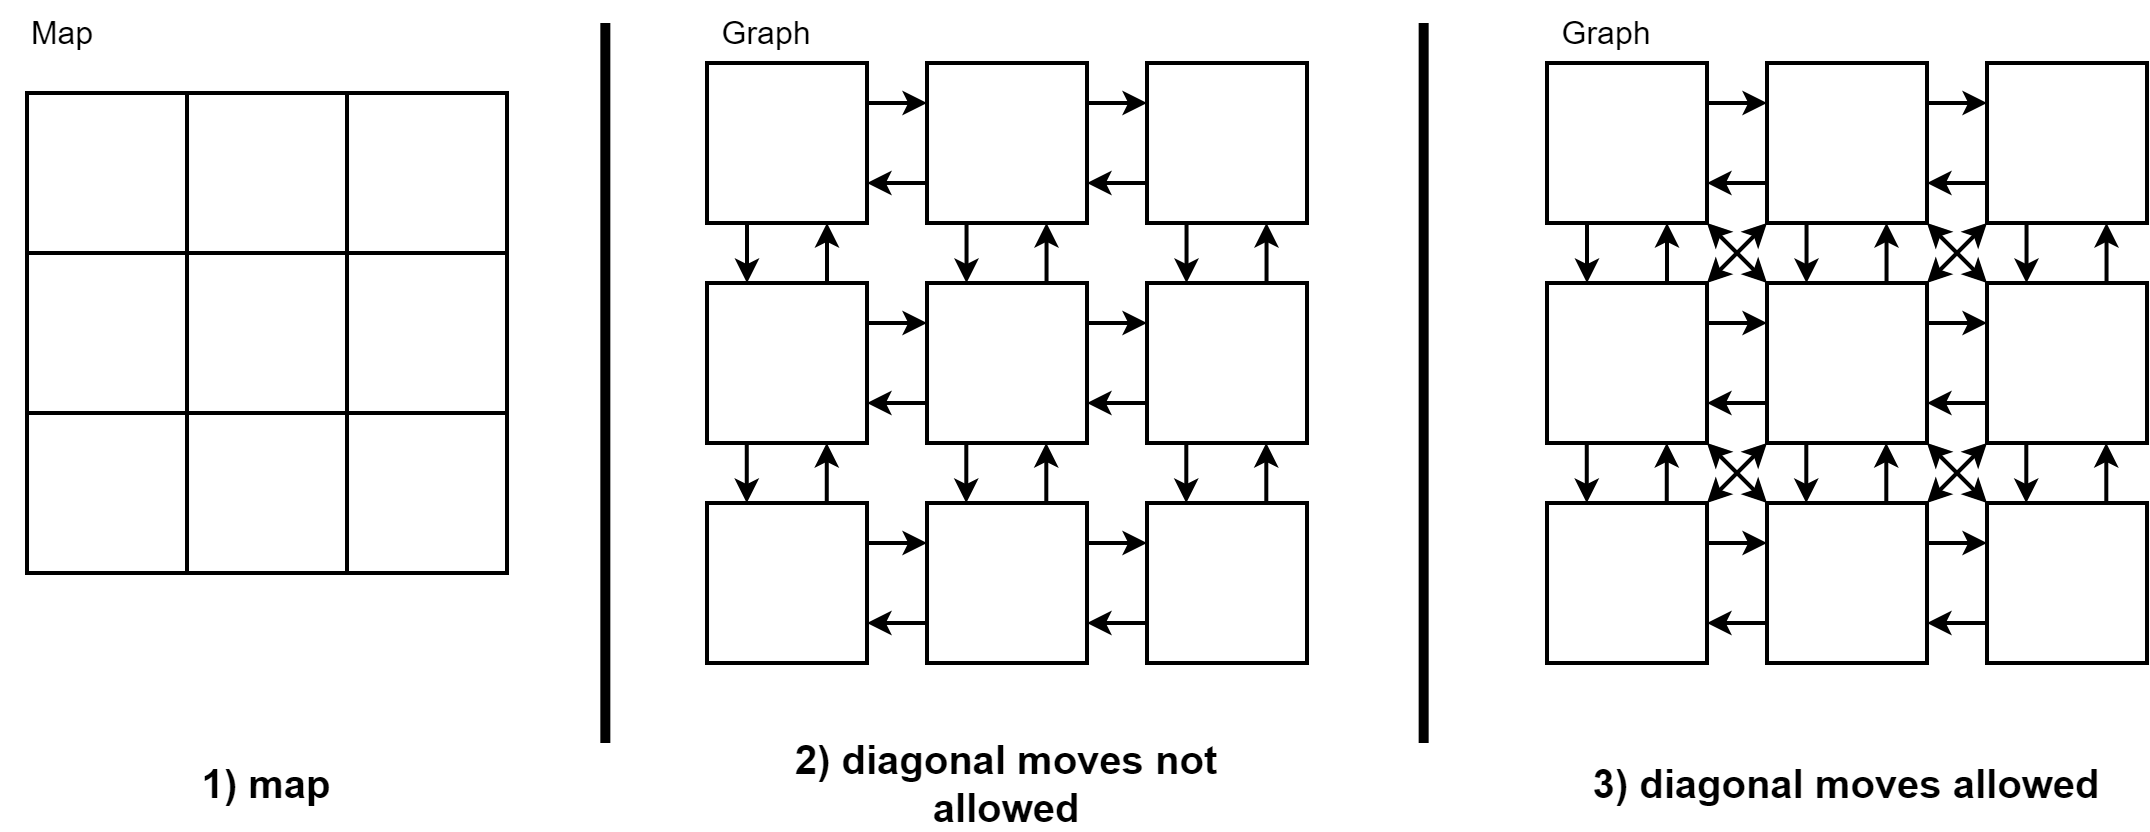
\includegraphics[width=\textwidth]{pictures/map_2d.png}
    \caption{ 2D map to graph translation }
    \label{fig:map_2D}
\end{figure}


\subsection{Gridmap for CA* algorithm}
For CA* algorithm map has to be translated into 3d gridmap where every layer is a representation of possible location of the agent in particular time-frame and therefore time becomes third dimension in a graph. Similar as in 2d gridmap there are two possible modes which are represented on figure below.
\begin{figure}[H]
    \centering
    \includegraphics[width=\textwidth]{pictures/map_3D.png}
    \caption{ 3D map to graph translation }
    \label{fig:map_3D}
\end{figure}

\subsection{CA* front collision problem}

\begin{figure}[H]
    \centering
    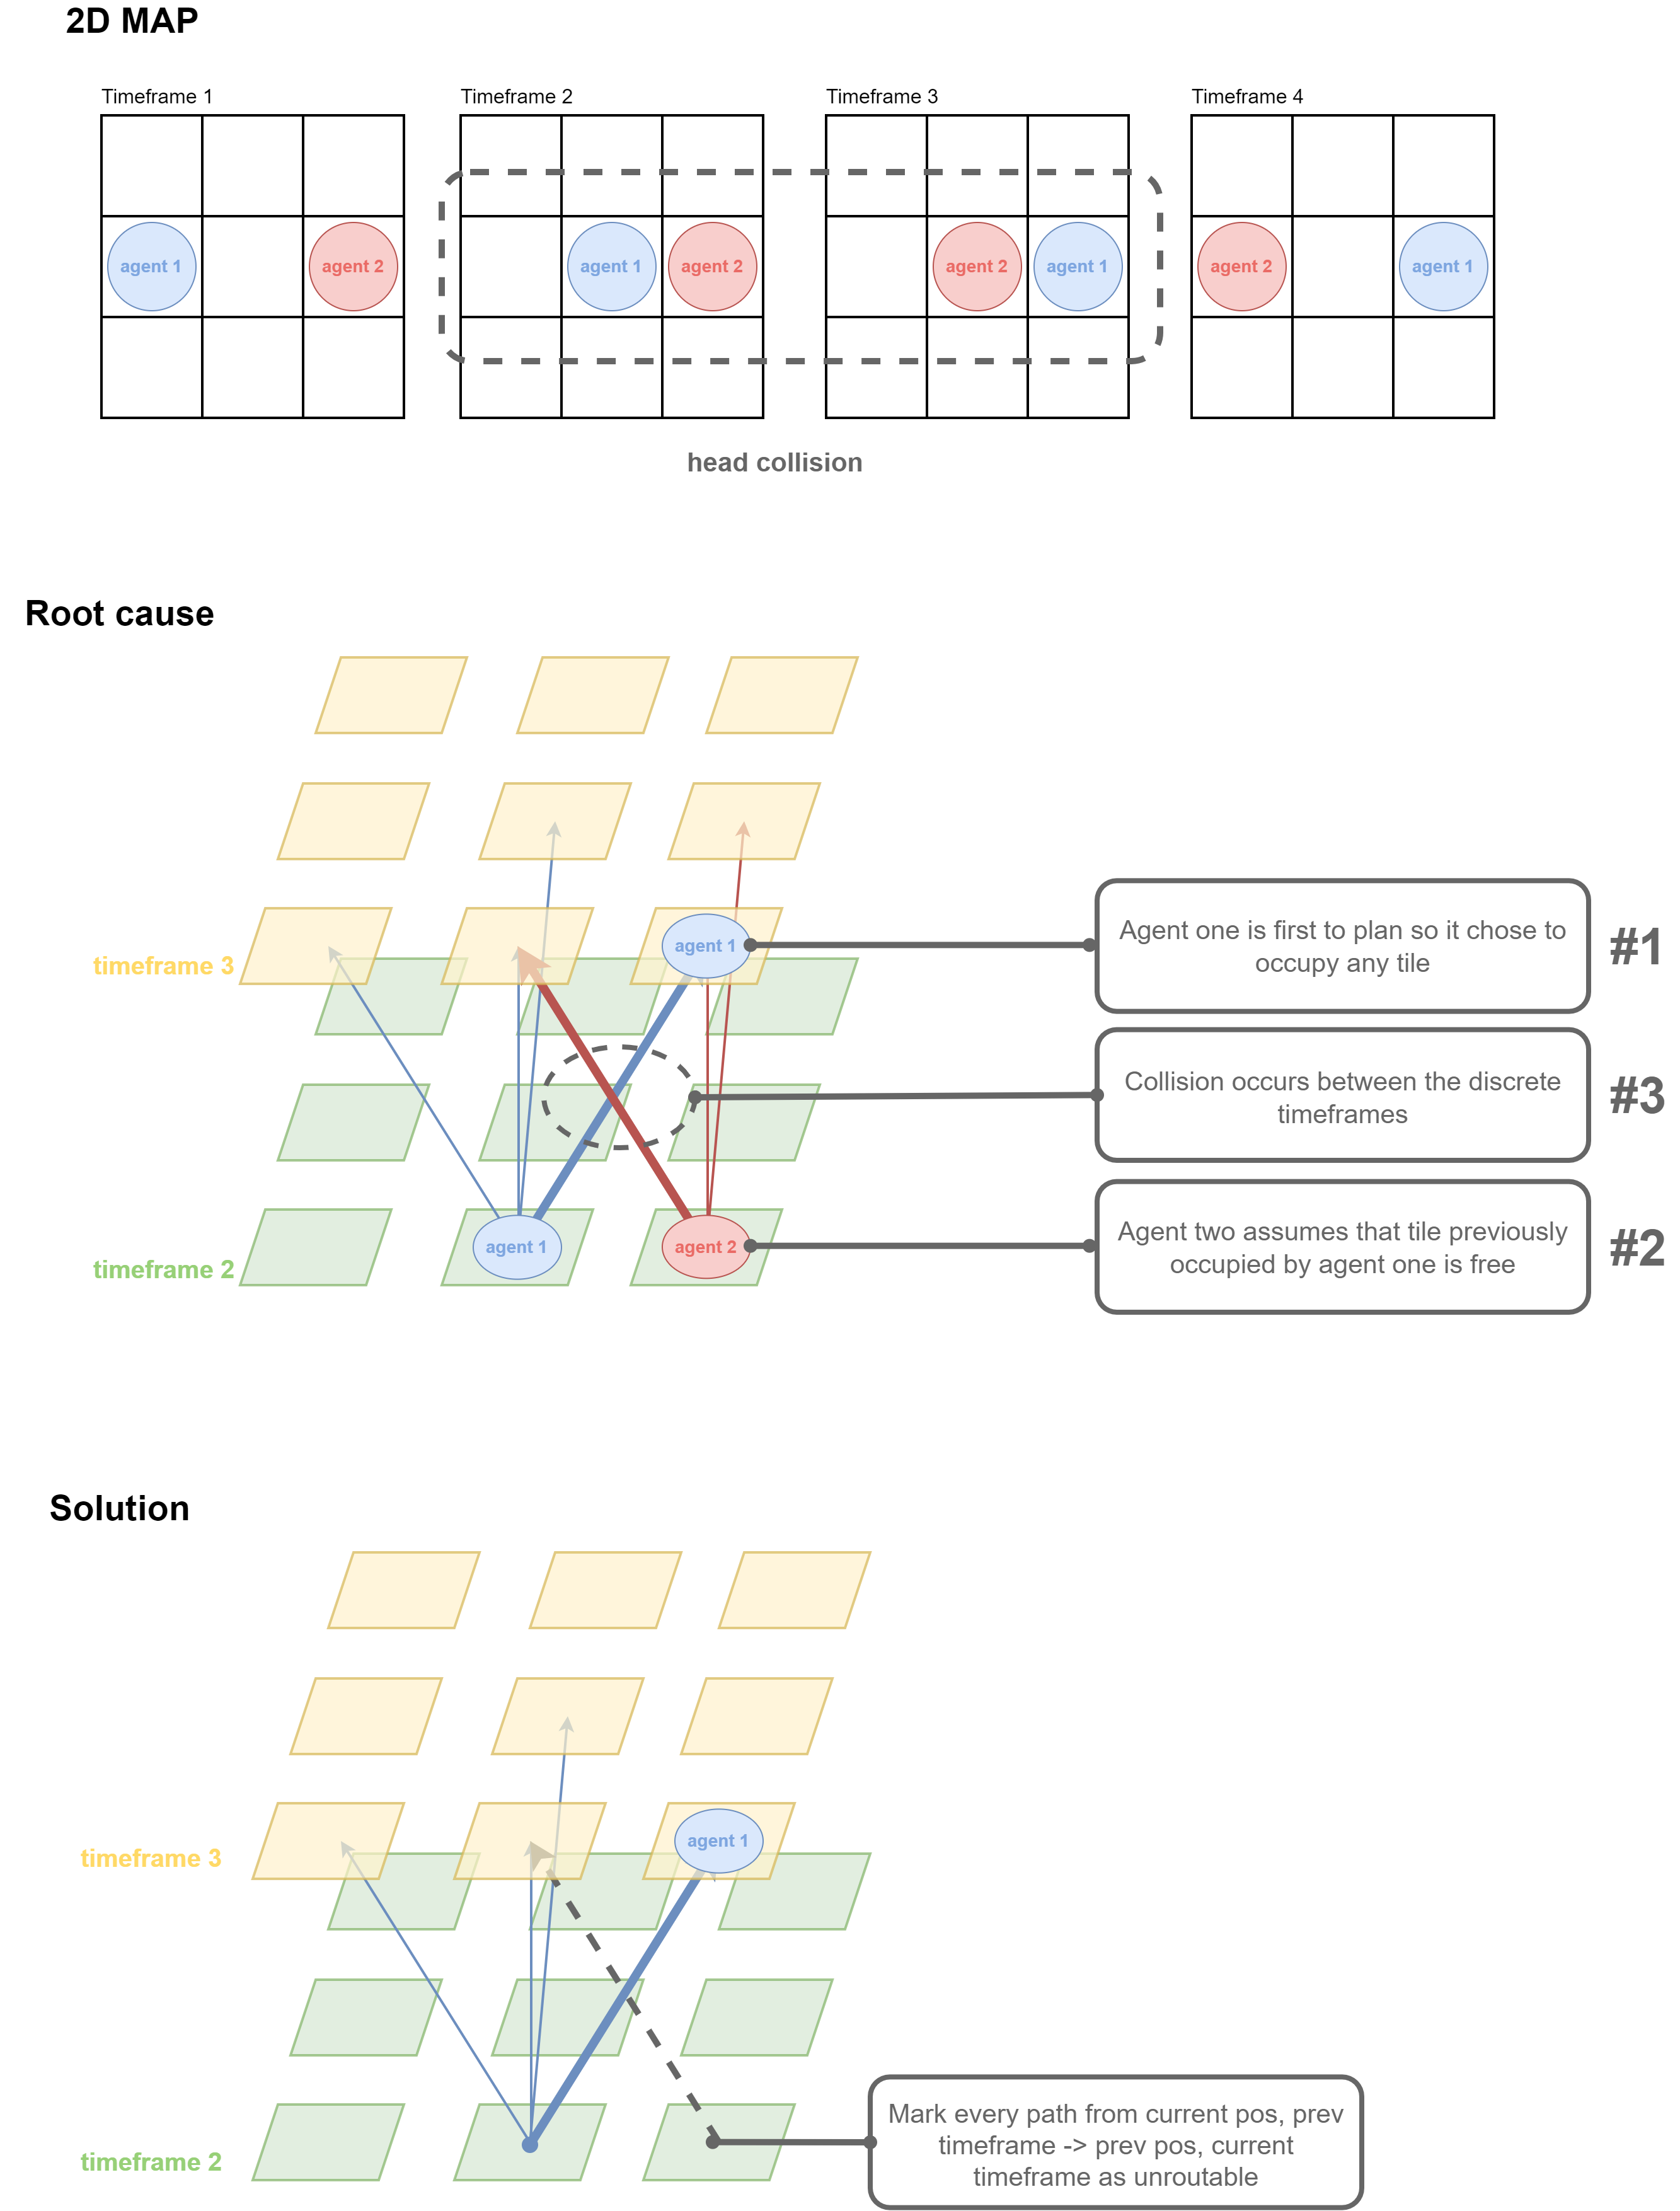
\includegraphics[width=\textwidth]{pictures/head_collision_problem.png}
    \caption{ CA* head collision problem}
    \label{fig:head_collision}
\end{figure}